%%%%%%%%%%%%%%%%%%%%%%%%%%%%%%%%%%%%%%%%%%%%%%%%%%%%%%%%%%%%
%%  This Beamer template was created by Cameron Bracken.
%%  Anyone can freely use or modify it for any purpose
%%  without attribution.
%%
%%  Last Modified: January 9, 2009
%%
%% https://www.sharelatex.com/templates/presentations/cameron-bracken-beamer/
%%

\documentclass[xcolor=x11names,compress]{beamer}

%% General document %%%%%%%%%%%%%%%%%%%%%%%%%%%%%%%%%%
\usepackage{graphicx}
\usepackage{tikz}
\usetikzlibrary{decorations.fractals}
%%%%%%%%%%%%%%%%%%%%%%%%%%%%%%%%%%%%%%%%%%%%%%%%%%%%%%


%% Beamer Layout %%%%%%%%%%%%%%%%%%%%%%%%%%%%%%%%%%
\useoutertheme[subsection=false,shadow]{miniframes}
\useinnertheme{default}
\usefonttheme{serif}
\usepackage{palatino}

\setbeamerfont{title like}{shape=\scshape}
\setbeamerfont{frametitle}{shape=\scshape}

\setbeamercolor*{lower separation line head}{bg=DeepSkyBlue4} 
\setbeamercolor*{normal text}{fg=black,bg=white} 
\setbeamercolor*{alerted text}{fg=red} 
\setbeamercolor*{example text}{fg=black} 
\setbeamercolor*{structure}{fg=black} 
 
\setbeamercolor*{palette tertiary}{fg=black,bg=black!10} 
\setbeamercolor*{palette quaternary}{fg=black,bg=black!10} 

\renewcommand{\(}{\begin{columns}}
\renewcommand{\)}{\end{columns}}
\newcommand{\<}[1]{\begin{column}{#1}}
\renewcommand{\>}{\end{column}}
%%%%%%%%%%%%%%%%%%%%%%%%%%%%%%%%%%%%%%%%%%%%%%%%%%

\begin{document}

%%%%%%%%%%%%%%%%%%%%%%%%%%%%%%%%%%%%%%%%%%%%%%%%%%%%%%
%%%%%%%%%%%%%%%%%%%%%%%%%%%%%%%%%%%%%%%%%%%%%%%%%%%%%%
\section{\scshape Introduction}
\begin{frame}
\title{Final Year Project}
\subtitle{Effects of ISI on Equal Gain Combining and Maximal-Ratio Combining with Sub-Optimal Design}
\author{
	Yann Donnelly\\
	{\it University College Cork}\\
}
\date{
	\vspace{1cm}
	7th February 2014
}
\titlepage
\end{frame}

%%%%%%%%%%%%%%%%%%%%%%%%%%%%%%%%%%%%%%%%%%%%%%%%%%%%%%
%%%%%%%%%%%%%%%%%%%%%%%%%%%%%%%%%%%%%%%%%%%%%%%%%%%%%%
%\subsection{Pointers}
%\begin{frame}{Pointers}
%\begin{itemize}
%\item 15 mins - 12 mins presentation, 3 mins questions
%\begin{itemize}
%\item brief context,  theory
%\item project aims and goals
%\item work acheived to date
%\item problems and solutions
%\item work to be performed
%\end{itemize}
%\item 1 slide per minute
%\item large fonts
%\item avoid formulae, complex diagrams
%\item uncluttered slides with block diagrams and lists are good
%\end{itemize}
%\end{frame}

%%%%%%%%%%%%%%%%%%%%%%%%%%%%%%%%%%%%%%%%%%%%%%%%%%%%%%
%%%%%%%%%%%%%%%%%%%%%%%%%%%%%%%%%%%%%%%%%%%%%%%%%%%%%%
\begin{frame}{Introduction}
\tableofcontents
\end{frame}

%%%%%%%%%%%%%%%%%%%%%%%%%%%%%%%%%%%%%%%%%%%%%%%%%%%%%%
%%%%%%%%%%%%%%%%%%%%%%%%%%%%%%%%%%%%%%%%%%%%%%%%%%%%%%
\section{\scshape Background}
\subsection{Communications Overview}
\begin{frame}{A Typical Communications System}
\begin{figure}[h!]
  \centering
    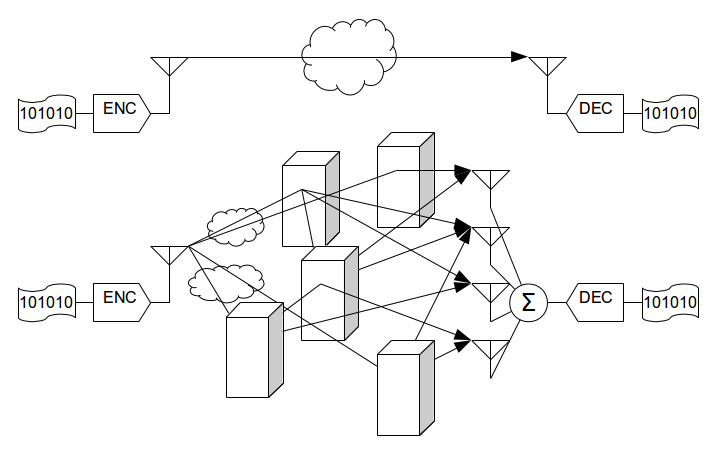
\includegraphics[width=\textwidth]{comms.png}
\end{figure}
%\emph{Image of typical comms system}
\end{frame}

%%%%%%%%%%%%%%%%%%%%%%%%%%%%%%%%%%%%%%%%%%%%%%%%%%%%%%
%%%%%%%%%%%%%%%%%%%%%%%%%%%%%%%%%%%%%%%%%%%%%%%%%%%%%%
\subsection{Detection Basics}
\begin{frame}{Detection Basics}
Likelihood of receiving a signal
\begin{figure}[h!]
  \centering
    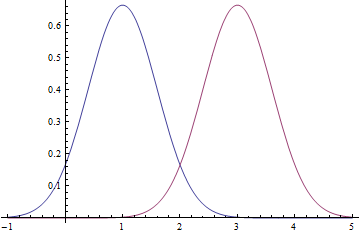
\includegraphics[width=0.8\textwidth]{../../plots/seminar_gaussian_sync.png}
%\emph{Image of received signal PDF}
\end{figure}
\end{frame}

%%%%%%%%%%%%%%%%%%%%%%%%%%%%%%%%%%%%%%%%%%%%%%%%%%%%%%
%%%%%%%%%%%%%%%%%%%%%%%%%%%%%%%%%%%%%%%%%%%%%%%%%%%%%%
\begin{frame}{Detection Basics}
Received signal response
\begin{figure}[h!]
  \centering
    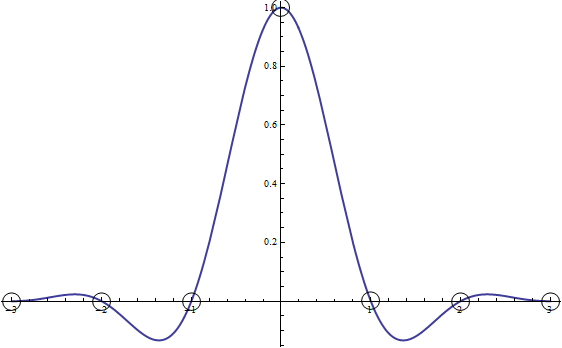
\includegraphics[width=0.8\textwidth]{../../plots/seminar_rrc_sync.png}
\end{figure}
%\emph{Image of RRC response}
\end{frame}

%%%%%%%%%%%%%%%%%%%%%%%%%%%%%%%%%%%%%%%%%%%%%%%%%%%%%%
%%%%%%%%%%%%%%%%%%%%%%%%%%%%%%%%%%%%%%%%%%%%%%%%%%%%%%
\begin{frame}{Detection Basics}
Received signal response with timing error
\begin{figure}[h!]
  \centering
    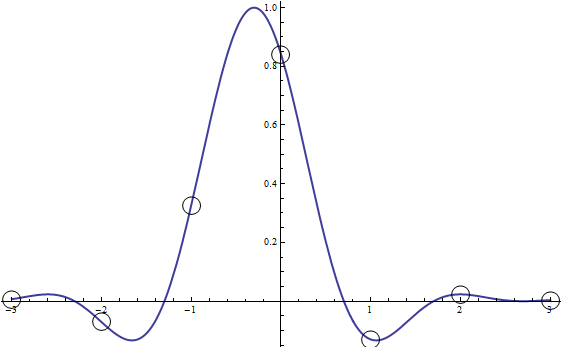
\includegraphics[width=0.8\textwidth]{../../plots/seminar_rrc_error.png}
\end{figure}
%\emph{Image of RRC response with offset}
\end{frame}

%%%%%%%%%%%%%%%%%%%%%%%%%%%%%%%%%%%%%%%%%%%%%%%%%%%%%%
%%%%%%%%%%%%%%%%%%%%%%%%%%%%%%%%%%%%%%%%%%%%%%%%%%%%%%
\begin{frame}{Detection Basics}
Likelihood of receiving a signal
\begin{figure}[h!]
  \centering
    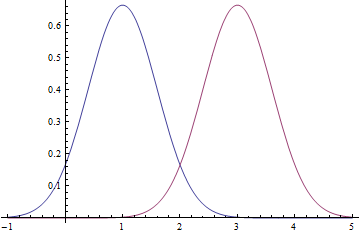
\includegraphics[width=0.8\textwidth]{../../plots/seminar_gaussian_sync.png}
\end{figure}
%\emph{Image of received signal PDF}
\end{frame}

%%%%%%%%%%%%%%%%%%%%%%%%%%%%%%%%%%%%%%%%%%%%%%%%%%%%%%
%%%%%%%%%%%%%%%%%%%%%%%%%%%%%%%%%%%%%%%%%%%%%%%%%%%%%%
\begin{frame}{Detection Basics}
Likelihood of receiving a signal with timing error
\begin{figure}[h!]
  \centering
    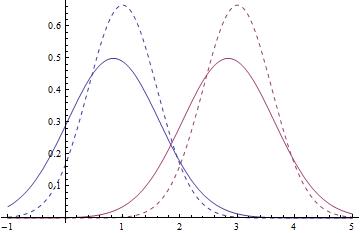
\includegraphics[width=0.8\textwidth]{../../plots/seminar_gaussian_error.png}
\end{figure}
%\emph{Image of received signal PDF with offset}
\end{frame}

%%%%%%%%%%%%%%%%%%%%%%%%%%%%%%%%%%%%%%%%%%%%%%%%%%%%%%
%%%%%%%%%%%%%%%%%%%%%%%%%%%%%%%%%%%%%%%%%%%%%%%%%%%%%%
\subsection{Aims of Project}
\begin{frame}{Aims of Project}
To determine the effects of Tikhonov-distributed timing offset on receiver performance, and develop a means of improving performance through redefining the decision region boundaries.
\end{frame}

%%%%%%%%%%%%%%%%%%%%%%%%%%%%%%%%%%%%%%%%%%%%%%%%%%%%%%
%%%%%%%%%%%%%%%%%%%%%%%%%%%%%%%%%%%%%%%%%%%%%%%%%%%%%%
\section{\scshape Results}
\subsection{Achievements}
\begin{frame}{Achievements}
\begin{itemize}
\item<2-> Developed models of 4-PAM communications systems in Mathematica
\item<3-> Examined performance in non-fading (line-of-sight) environment
\item<4-> Examined performance in Rayleigh fading environment with EGC
\item<5-> Examined performance in Rayleigh fading environment with MRC
\item<6-> Positive results:
	\begin{itemize}
	\item Lower optimum decision region boundaries in the presence of timing error
	\item Performance increase from redesigning detector to take this into account
	\end{itemize}
\end{itemize}
\end{frame}

%%%%%%%%%%%%%%%%%%%%%%%%%%%%%%%%%%%%%%%%%%%%%%%%%%%%%%
%%%%%%%%%%%%%%%%%%%%%%%%%%%%%%%%%%%%%%%%%%%%%%%%%%%%%%
\subsection{Results}
\begin{frame}{Results}
\begin{itemize}
\item EGC: Improvements of 20-33\%
\item MRC: Improvements of 7-20\%
\end{itemize}
\begin{figure}[h!]
  \centering
    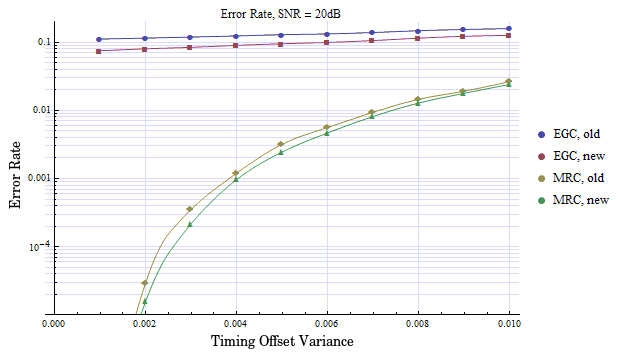
\includegraphics[width=0.9\textwidth]{egc_mrc_cropped.png}
\end{figure}
%\emph{Plot of ER}
\end{frame}

%%%%%%%%%%%%%%%%%%%%%%%%%%%%%%%%%%%%%%%%%%%%%%%%%%%%%%
%%%%%%%%%%%%%%%%%%%%%%%%%%%%%%%%%%%%%%%%%%%%%%%%%%%%%%
\section{\scshape Obstacles}
\subsection{Problems Encountered}
\begin{frame}{Problems Encountered}
\begin{itemize}
\item<2-> Simulation speed: 6 ways to do anything, only one is “fast”
	\begin{itemize}
	\item Solution: Read up on Mathematica functions, testing and timing each method
	\item Solution: Reduce how often you have to do something
	\item Solution: Functions with memory
	\item Solution: Parallel computing
	\end{itemize}
\item<3-> Running simulations across multiple headless machines
	\begin{itemize}
	\item Solution: Remote access
	\end{itemize}
\item<4-> Running simulations across multiple machines that can be switched off at any point
	\begin{itemize}
	\item Solution: Output regularly
	\item Solution: Make sure outputs are descriptive
	\item Solution: Easily reconfigurable code
	\end{itemize}
\end{itemize}
\end{frame}

%%%%%%%%%%%%%%%%%%%%%%%%%%%%%%%%%%%%%%%%%%%%%%%%%%%%%%
%%%%%%%%%%%%%%%%%%%%%%%%%%%%%%%%%%%%%%%%%%%%%%%%%%%%%%
\section{\scshape Future Work}
\subsection{Future Work}
\begin{frame}{Future Work}
\begin{itemize}
\item<2-> Describe the effects of timing error offset analytically
\item<3-> Determine the Gram-Charlier PDF approximation
\item<4-> Summarize findings in a publication
\end{itemize}
\end{frame}

\end{document}